\documentclass[fleqn, xcolor=x11names]{beamer}
\usetheme{Frankfurt} % шаблон
\usecolortheme{default} % цветовая схема
\usepackage[11pt]{moresize}
\usepackage{multimedia}
\usepackage[T1]{fontenc}
\usepackage{pgfplots}
\usepackage[utf8]{inputenc}
\usepackage[russian]{babel}
\usepackage{media9}
\usepackage{listings}
\usepackage{amsmath}
\usepackage{color}
\usepackage{parskip}

\usepackage{graphicx}
\lstdefinestyle{myLatexStyle}{
    basicstyle=\small\ttfamily,
    language={python},
    numbersep=5mm, numbers=left, numberstyle=\tiny, % number style
    breaklines=true,frame=single,framexleftmargin=8mm, xleftmargin=8mm,
    backgroundcolor=\color{green!5}, frameround=fttt,escapeinside=??,
    rulecolor=\color{red},
    morekeywords={% Give keywords here
        numpy},
    keywordstyle=\color[rgb]{0,0,1},                    % keywords
        commentstyle=\color[rgb]{0.133,0.545,0.133},    % comments
        stringstyle=\color[rgb]{0.627,0.126,0.941}  % strings
}
\lstset{style=myLatexStyle}

\setbeamertemplate{navigation symbols}{}
\setbeamertemplate{footline}{%
    \hspace{0.99\paperwidth}%
    \usebeamerfont{title in head/foot}%
    \insertframenumber\,/\,\inserttotalframenumber%
}


\title{Meta-learning}
\author[Медведев~Д.\,В.]{Медведев Алексей Владимирович}
\institute[ВМК МГУ]{МГУ имени М. В. Ломоносова,
факультет ВМК, кафедра ММП}
\date{} 

\begin{document}

\begin{frame}
\maketitle
\end{frame}

\begin{frame}
\begin{block}{Meta-learning}
Многообещающая область машинного обучения. Стандартного определения пока что нет, но идея состоит в том, что мы строим систему, которая может улучшить качество алгоритма при решении конкретной задачи, или адаптировать алгоритм для решения новых задач. Можно сказать, что ставится задача научиться учить (learn-to-learn). Аналогия "--- эволюционный процесс, создавший человеческий мозг.
\end{block}
\end{frame}



\begin{frame}[fragile]\frametitle{Neural Architecture Search}

\begin{block}{Проблема}

Нейронные сети хорошо показали себя в задачах обработки изображений, речи, понимания языка. Но конструирование нейросети остается непростой задачей, требующей определенных навыков.
\end{block}

\begin{block}{Идея}
Создать алгоритм, который сможет описывать архитектуру нейросети для данной задачи машинного обучения.

\end{block}

\end{frame}

\begin{frame}[fragile]\frametitle{Neural Architecture Search}

\begin{block}{Neural Architecture Search [Barret Zoph, Quoc V. Le 2017]}

\begin{itemize}
\item Архитектура нейросети может быть записана как строка произвольной длины

\item Можно взять RNN (controller), каждый блок которой будет отвечать за определенный параметр искомой архитектуры(Количество фильтров в слое сверточной нейросети, с какими слоями соединен данный слой(skip connections) и т.д.)

\item Обучить controller с помощью Reinforcement-learning, считая что вознаграждение это точность полученной архитектуры на кросс-валидации.
\end{itemize}

\end{block}


\end{frame}


\begin{frame}[fragile]\frametitle{REINFORCE}

\begin{block}{REINFORCE algorithms [Williams, 1992]}

Чтобы найти оптимальный алгоритм с точки зрения reinforcement-learning необходимо максимизировать мат.ожидание награды: $J(\theta) = E_{\pi_{\theta}} [R]$.

Где $\pi_{\theta}$ "--- policy функция, по сути и есть алгоритм, который мы обучаем.
 
Зачастую функция вознаграждения(R) недеффиринцируема, поэтому было придумано множество REINFORCE правил, которые позволяют применить градиентный спуск напрямую к policy-function.

 Эти правила в общем виде можно записать так:
\begin{center}
$\Delta \theta = \alpha \nabla \log{(\pi_{\theta})}(r-b)$
\end{center}

Где $r$ "--- текущий reward, $b$ "--- baseline(скользящее среднее предыдущих вознаграждений), $\alpha$ - learning rate.


\end{block}

\end{frame}

\begin{frame}[fragile]\frametitle{Neural Architecture Search}
\begin{figure}[h]
\begin{center}
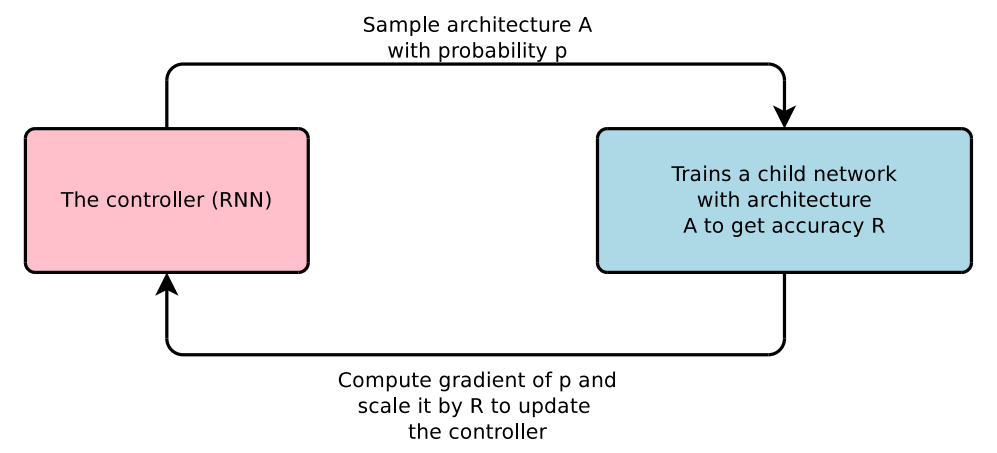
\includegraphics[scale=0.4]{/home/alex/python/D'yakonov/nas_scheme.png}
\caption{Итоговый алгоритм обучения controller-network}
\end{center}
\end{figure}
\end{frame}

\begin{frame}[fragile]\frametitle{Neural Architecture Search}

\begin{block}{Итоговый алгоритм}
С помощью вышеупомянутого REINFORCE rule градиент нашего функционала принимает следующий вид:
\begin{center}
$ \nabla_{\theta_c} J(\theta_c) = \frac{1}{m}\sum \limits_{k=1}^m  \sum \limits_{t=1}^T \nabla_{\theta_c} \log{P(a_t | a_{(t-1):1}; \theta_c)}(R_k-b)$
\end{center}

Где $m$ --- размер batch'a, созданных controller'ом архитектур, 

$R_k$ --- вознаграждение, которое получено для данной архитектуры, 

$T$ --- количество гиперпараметров, которые controller должен определить,

$P$ --- вероятностная модель, которую моделирует controller.
\end{block}
\end{frame}

\begin{frame}\frametitle{Neural Architecture Search}

\begin{figure}[h]
\begin{center}
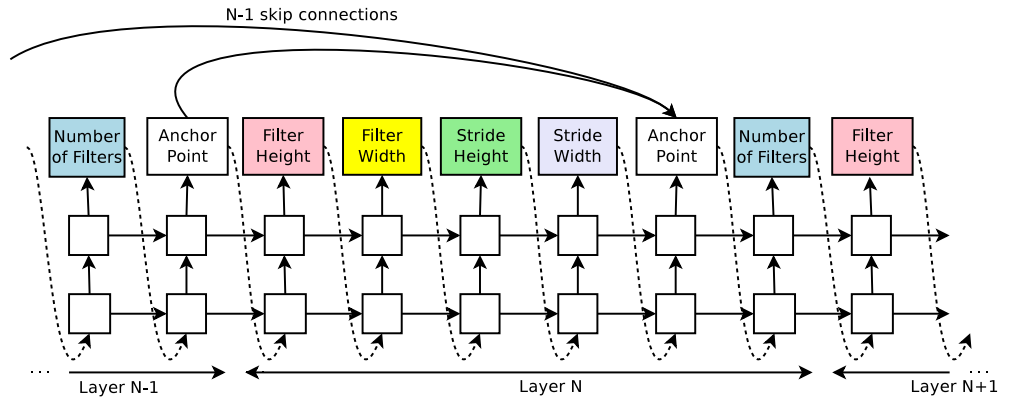
\includegraphics[scale=0.22]{/home/alex/python/D'yakonov/nas_architecture.png}
\caption{Пример архитектуры controller'a, ищущего архитектуру сверточной нейросети.}
\end{center}
\end{figure}

\begin{figure}[h]
\begin{center}
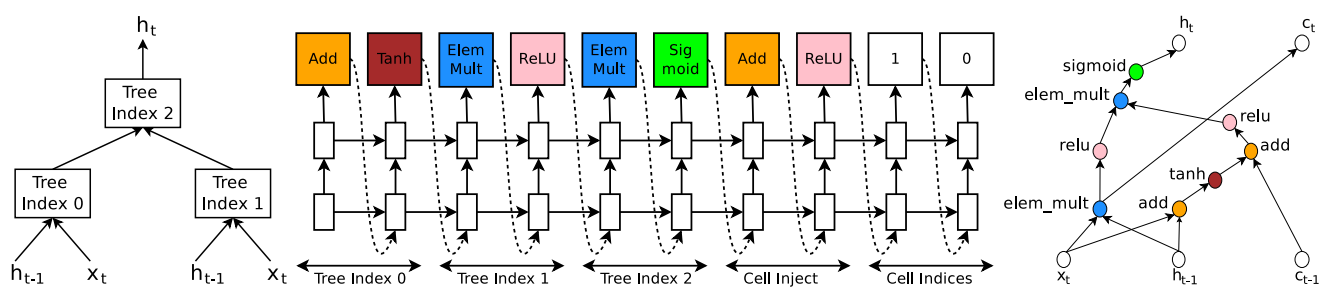
\includegraphics[scale=0.25]{/home/alex/python/D'yakonov/nas_rnn_architecture.png}
\caption{Пример архитектуры controller'a, ищущего архитектуру, рекуррентной нейросети.}
\end{center}
\end{figure}


\end{frame}

\begin{frame}\frametitle{Neural Architecture Search}

\begin{block}{Архитектура controller'a}
Controller представляет собой RNN, каждый выход которой представляет собой выход softmax классификатора и подается на вход следующему блоку. Каждый блок предсказывает свой параметр конструируемой архитектуры, такие блоки можно сгруппировать по слоям будущей нейросети. В более сложном случае появляются особые блоки, которые отвечают за skip-connections.

Особый случай представляет конструирование рекуррентных нейросетей, блоки на выходе предсказывают функции активации, опреации над внутренней памятью и входом блока рекуррентной нейросети.
\end{block}

\end{frame}

\begin{frame}\frametitle{Neural Architecture Search}

\begin{figure}[h]
\begin{center}
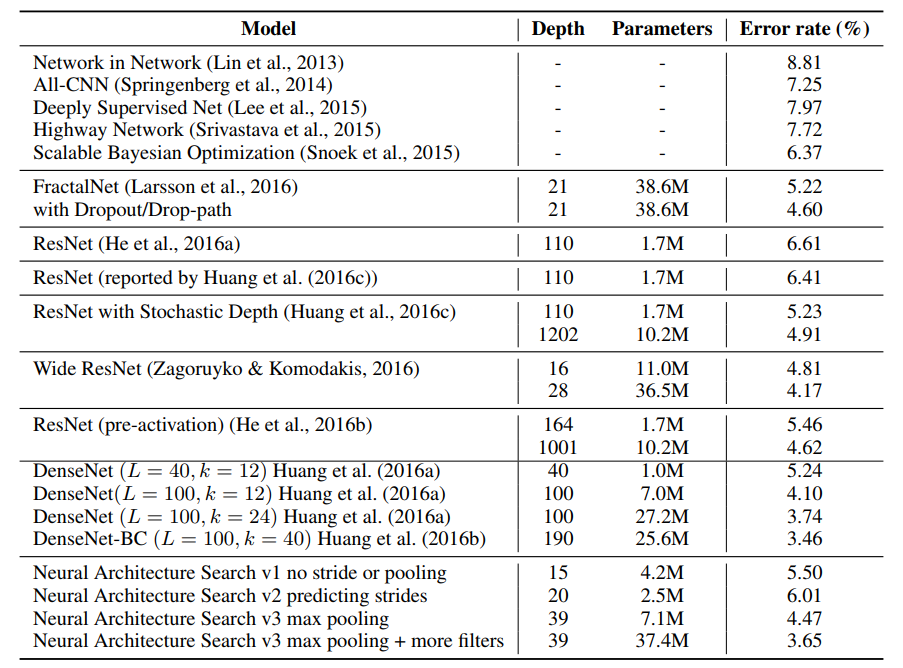
\includegraphics[scale=0.35]{/home/alex/python/D'yakonov/nas_cifar10.png}
\caption{Результаты state-of-the-art моделей и найденных алгоритмом архитектур на датасете CIFAR10(классификация).}
\end{center}
\end{figure}

\end{frame}


\begin{frame}\frametitle{Neural Architecture Search}

\begin{figure}[h]
\begin{center}
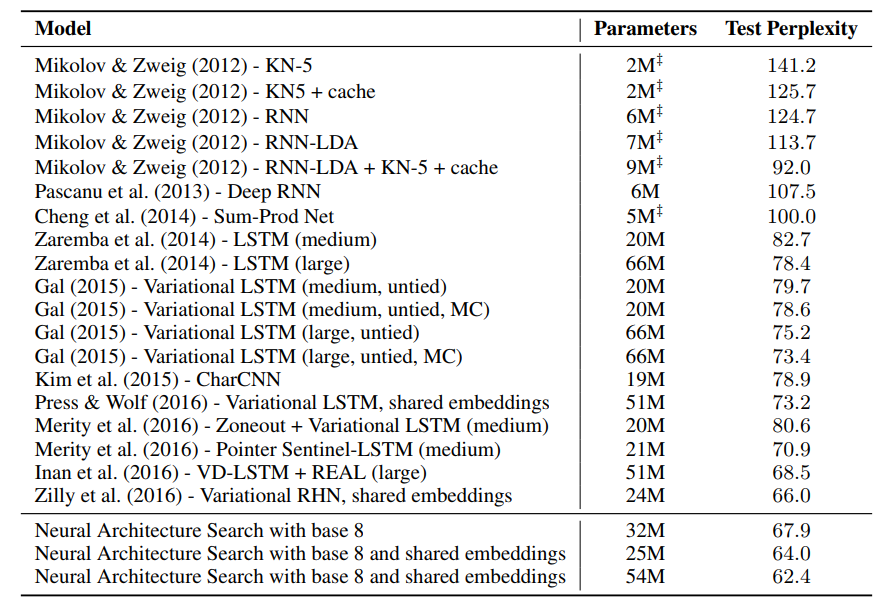
\includegraphics[scale=0.35]{/home/alex/python/D'yakonov/nas_ptb.png}
\caption{Результаты state-of-the-art моделей и найденных алгоритмом архитектур на датасете  Penn Treebank.}
\end{center}
\end{figure}

\end{frame}

\begin{frame}\frametitle{Neural Architecture Search}




\begin{block}{Результат}
{\footnotesize Алгоритм нашел несколько интересных архитектур как в случае классификации, так и в случае более сложной задачи моделирования языка. Более того последние показали еще и хорошие результаты на задаче машинного перевода.}
\end{block}

\begin{table}[h]
\begin{center}
\begin{tabular}{*{3}{c}}

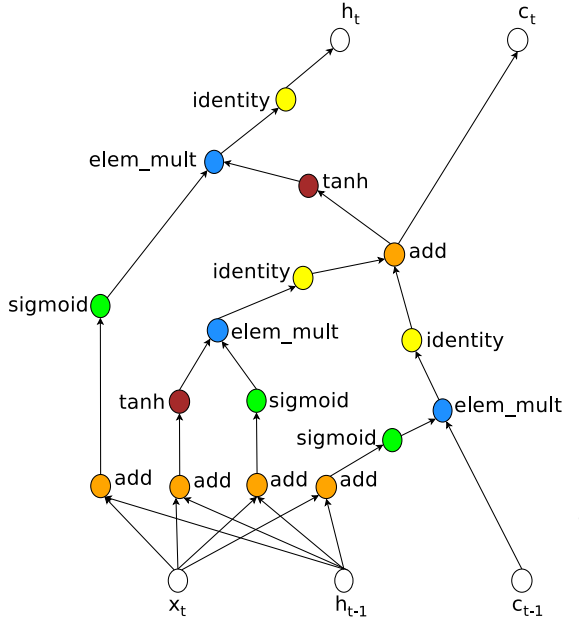
\includegraphics[width = 3cm]{/home/alex/python/D'yakonov/nas_lstm.png} &
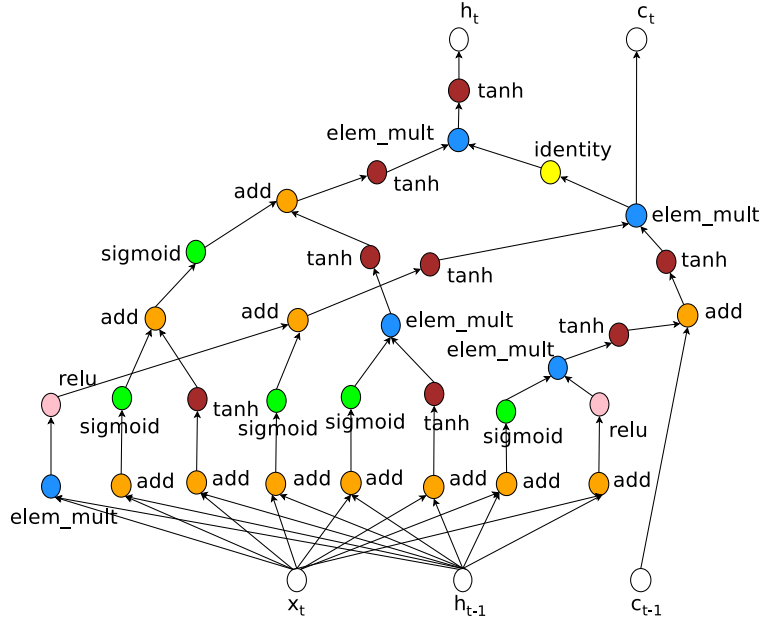
\includegraphics[width = 3cm]{/home/alex/python/D'yakonov/nas_new_cell.png} &
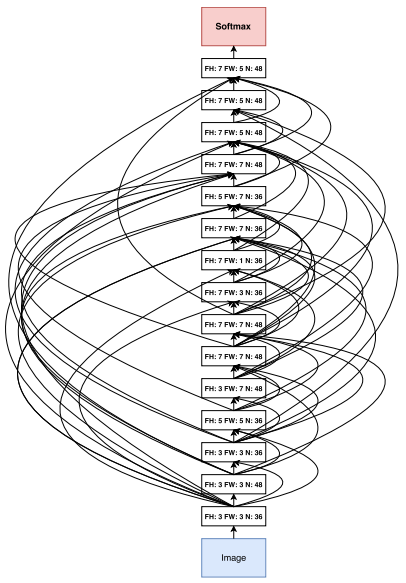
\includegraphics[scale = 0.2]{/home/alex/python/D'yakonov/nas_final1.png} \\

\end{tabular}
\caption{{\footnotesize LSTM и полученные модели: модуль рекуррентной нейросети и архитектура для CIFAR10}}
\end{center}
\end{table}

\end{frame}

\begin{frame}\frametitle{Sim2Real with meta learning}

\begin{block}{{\footnotesize Проблема}}
{\footnotesize Есть задачи, например создание автопилота для вертолета, обучение для которых в реальной жизни либо очень дорого, либо невозможно. В то же время обучение в симуляторе настоящей среды сопряжено с некоторыми проблемами. Чем полнее симуляция среды, тем она тяжелее с вычислительной точки зрения, а значит обучение будет проходить медленно, плюс обучаемые агенты могут использовать упрощения и баги симуляции для создания своих оптимальных, но неприменимых в реальной жизни стратегий. Хотелось бы уметь обучать агента в симуляторе, но так чтобы он преуспел в реальном мире.}
\end{block}

\begin{block}{{\footnotesize Идея}}

{\footnotesize Создать алгоритм, который будет адаптироваться к параметрам среды, в которой он действует. Для этого можно обучить алгоритм на симуляциях среды с рандомизированными параметрами.}

\end{block}

\end{frame}

\begin{frame}\frametitle{Sim2Real with meta learning}

\begin{block}{{\footnotesize Метод [Peng et al., 2017]}}
{\footnotesize
Наша цель натренировать policy функции, которые смогут решать задачи, в среде описанной динамикой реального мира $p^*(s_{t+1}|a_t, s_t)$. Но ее использование может быть накладным. Поэтому мы приближаем ее моделью $\hat{p}(s_{t+1}|a_t, s_t, \mu) \approx p^*(s_{t+1}|a_t, s_t)$. Где $\mu$ --- множество параметров(масса конечностей робота, масса и трение шайбы, высота стола и т.д). В таких терминах можно сформулировать задачу как максимизацию следующего функционала:
\begin{center}
$ E_{\mu \sim \rho_{\mu}} \left[ E_{\tau \sim p(\tau|\pi,\mu)} \left[  \sum \limits_{t=0}^{T-1} r(s_t, a_t) \right] \right]$
\end{center}
Действия агента напрямую зависят от параметров функции динамики среды ($\mu$). Т.е policy функция зависит от них. Если во время тренировки параметры $\mu$ нам известны, то в реальном мире дела обстоят сложнее. Предлагается оценивать эти параметры с помощью истории действий и состояний $h_t = [a_{t-1}, s_{t-1}, a_{t-2}, s_{t-2}...]$. Для этого сделаем функцию policy рекуррентной $\pi(a_t|s_t, z_t)$, где внутренняя память $z_t = z(h_t)$ и есть механизм, позволяющий определить параметры.
}
\end{block}

\end{frame}

\begin{frame}\frametitle{Recurrent Deterministic Policy Gradient(RDPG)}

\begin{block}{{\footnotesize Метод}}
{\footnotesize Для обучения рекуррентных policy функций есть специальный алгоритм. Чтобы его применить нужны две обучаемые функции: policy ($\pi(a_t|s_t, z_t)$), value или omniscient critic ($Q(s_t, a_t, y_t, \mu)$) . Где $y_t = y(h_t)$ --- внутренняя память. Формулы обновления весов будут приведены далее в описании общего алгоритма. Идея заключается в том, что value функция аппроксимирует скользящее среднее вознаграждения, и таким образом корректирует обучение policy. Value функция обновляется согласно равенству Беллмана.}
\end{block}

\end{frame}

\begin{frame}\frametitle{Hindsight Experience Replay}

\begin{figure}[h]
\begin{center}
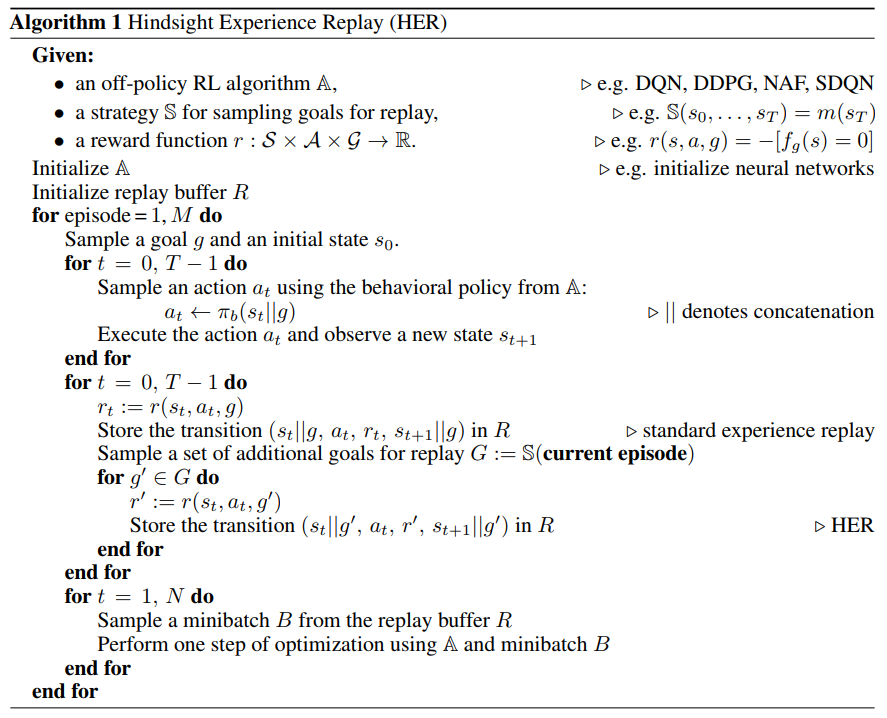
\includegraphics[scale=0.35]{/home/alex/python/D'yakonov/HER.png}
\caption{ Алгоритм, позволяющий справляться с разреженными функциями вознаграждений.}
\end{center}
\end{figure}

\end{frame}

\begin{frame}\frametitle{Sim2Real with meta learning}

\begin{figure}[h]
\begin{center}
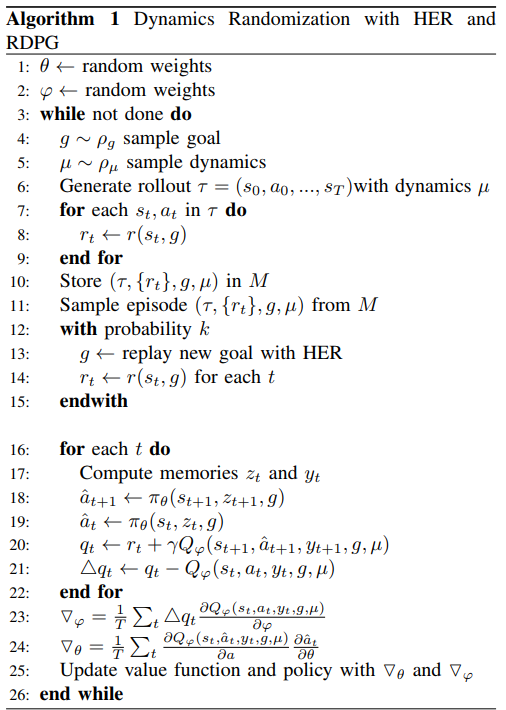
\includegraphics[scale=0.35]{/home/alex/python/D'yakonov/sim2real.png}
\caption{ Основной алгоритм обучения агента}
\end{center}
\end{figure}

\end{frame}


\begin{frame}\frametitle{Model-Agnostic Meta-Learning for Fast Adaptation of Deep Networks}

\begin{block}{Проблема}
{\footnotesize 
Случается так, что алгоритм должен уметь быстро, с очень небольшим количеством обучающих примеров, адаптироваться под решение новых задач. Например научить классифицировать изображения чайника, имея только пару его изображений, модель, которая уже умеет классифицировать множество объектов.
}
\end{block}

\begin{block}{Идея}
{\footnotesize 
Можно представить задачу следующим образом: модель $f$ работает с множеством задач $T$, имеющих некоторое распределение $p(T)$. Чтобы избежать переобучения и при этом решить новую задачу важно найти параметры модели, которые сильно влияют на функции потерь каждой задачи из $p(T)$. А так как не делается никаких предположений, кроме того, что модель параметризована, то данный подход можно обобщить на широкий круг задач от классификации до reinforcement learning. 
}
\end{block}

\end{frame}

\begin{frame}\frametitle{Model-Agnostic Meta-Learning for Fast Adaptation of Deep Networks}

\begin{figure}[h]
\begin{center}
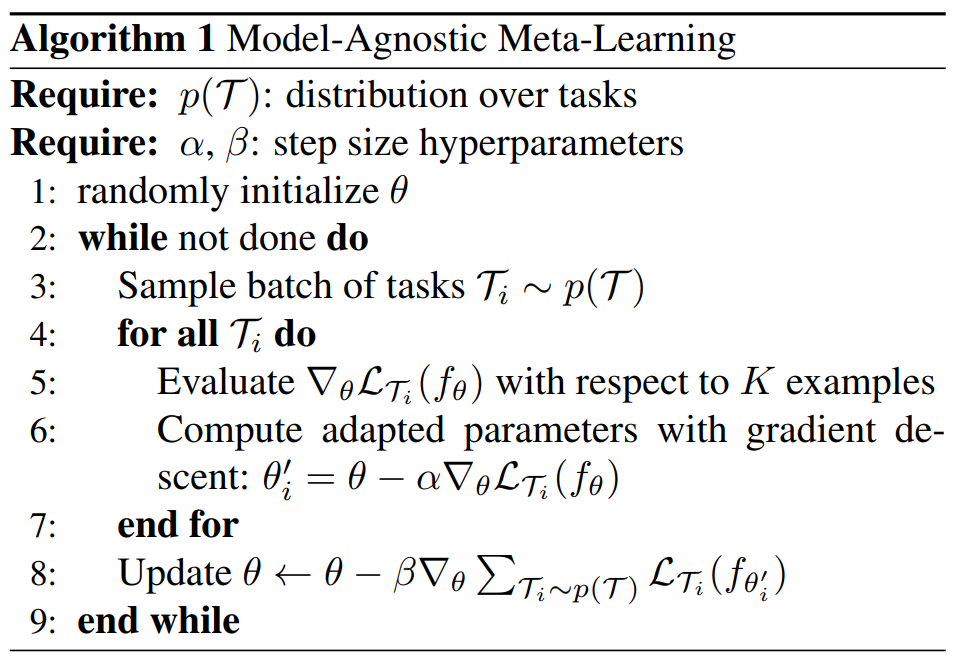
\includegraphics[scale=0.35]{/home/alex/python/D'yakonov/maml.png}
\caption{ Алгоритм MAML в общем виде}
\end{center}
\end{figure}

\end{frame}

\begin{frame}\frametitle{Model-Agnostic Meta-Learning for Fast Adaptation of Deep Networks}

\begin{figure}[h]
\begin{center}
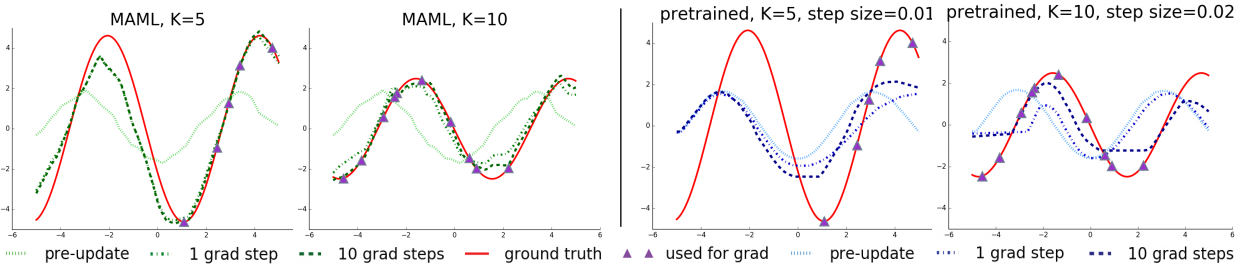
\includegraphics[scale=0.35]{/home/alex/python/D'yakonov/maml_regression.png}
\caption{{\footnotesize  Алгоритм MAML для регрессии}}
\end{center}
\end{figure}

\end{frame}
\begin{frame}\frametitle{Model-Agnostic Meta-Learning for Fast Adaptation of Deep Networks}

\begin{figure}[h]
\begin{center}
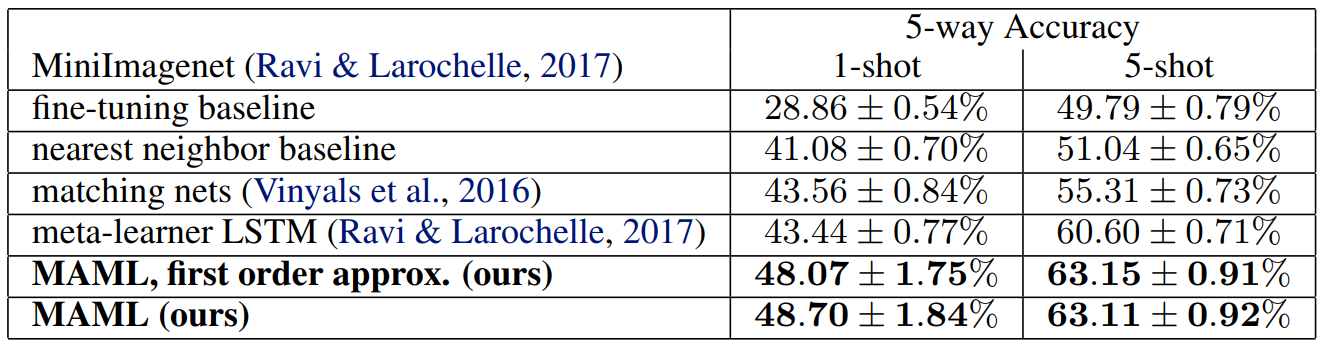
\includegraphics[scale=0.3]{/home/alex/python/D'yakonov/classification.png}
\caption{ Алгоритм MAML для классификации}
\end{center}
\end{figure}

\end{frame}

\begin{frame}\frametitle{Optimization as a model for few-shot learning}

\begin{block}{Идея}
{\footnotesize 
Создать модель, которая будет определять способ обновления параметров конечного алгоритма. Посмотрим на формулу градиентного спуска:
\begin{center}
 $ \theta_t = \theta_{t-1} - \alpha_t \nabla_{\theta_{t-1}}L_t$
\end{center}
Ключевым является следующее наблюдение. Формула обновления памяти ячейки LSTM сети (cell state) очень похожа на обновление параметров с помощью градиентного спуска:
\begin{center}
 $ c_t = f_t \odot c_{t-1} + i_t \odot \tilde{c}_t$
\end{center}
 Где $c_t$ будет играть роль параметров сети $\theta_t$ и $\tilde{c}_t = \nabla_{\theta_{t-1}}L_t$. В такой постановке $i_t$ будет обучаемым параметром:
\begin{center}
 $i_t = \sigma(W_I \cdot \left[ \nabla_{\theta_{t-1}}L_t, L_t, \theta_{t-1}, i_{t-1} \right] + b_I)$
 \end{center}
 Теперь learning rate является функцией от функции потерь, ее градиента, параметров сети и своего значения на предыдущем шаге. Константное занчение $f_t = 1$ кажется не самым оптимальным. Уменьшение параметров и забывание чати предыдущих их значений может оказаться полезным в точке неудачного локального оптимума. В ситуации когда значение градиента близко к нулю, а значение функции потерь довольно велико.
 \begin{center}
 $f_t = \sigma(W_F \cdot \left[ \nabla_{\theta_{t-1}}L_t, L_t, \theta_{t-1}, f_{t-1} \right] + b_F)$
\end{center}
}
\end{block}

\end{frame}



\begin{frame}\frametitle{Optimization as a model for few-shot learning}
\begin{figure}[h]
\begin{center}
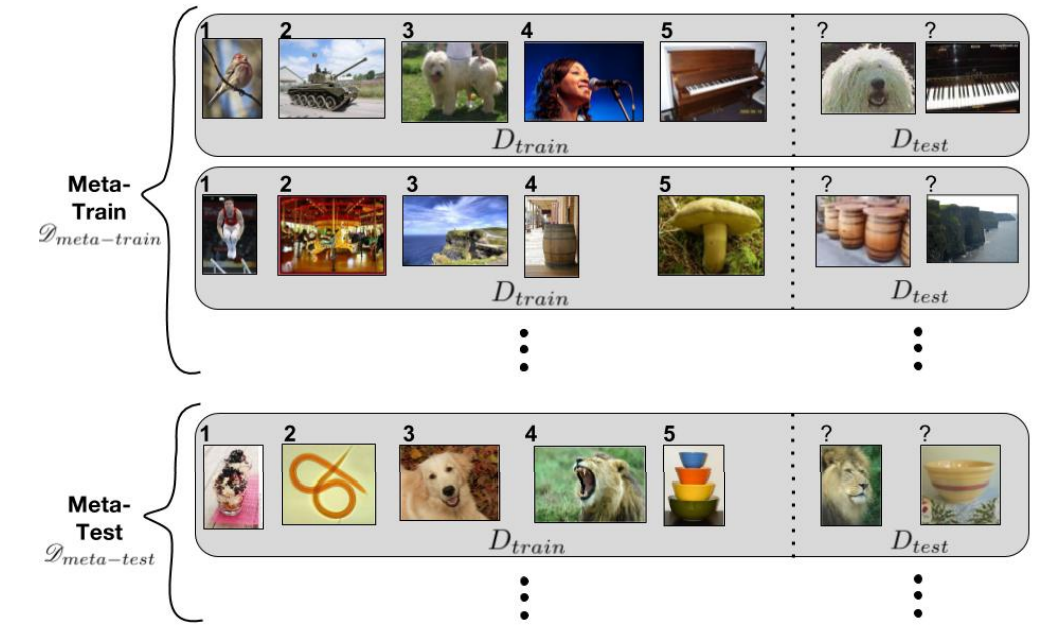
\includegraphics[scale=0.3]{/home/alex/python/D'yakonov/lstm_meta_sets.png}
\caption{{\footnotesize Обучение Meta-Learner'а происходит на множестве пар датасетов, называемых эпизодами. Каждая пара состоит из тренировочной и тестовой выборки. В тренировочной выборке присутствуют k*N элементов, где N --- количество классов, а k --- ограничение на количество элементов из одного класса. }}
\end{center}
\end{figure}
\end{frame}

\begin{frame}\frametitle{Optimization as a model for few-shot learning}

\begin{figure}[h]
\begin{center}
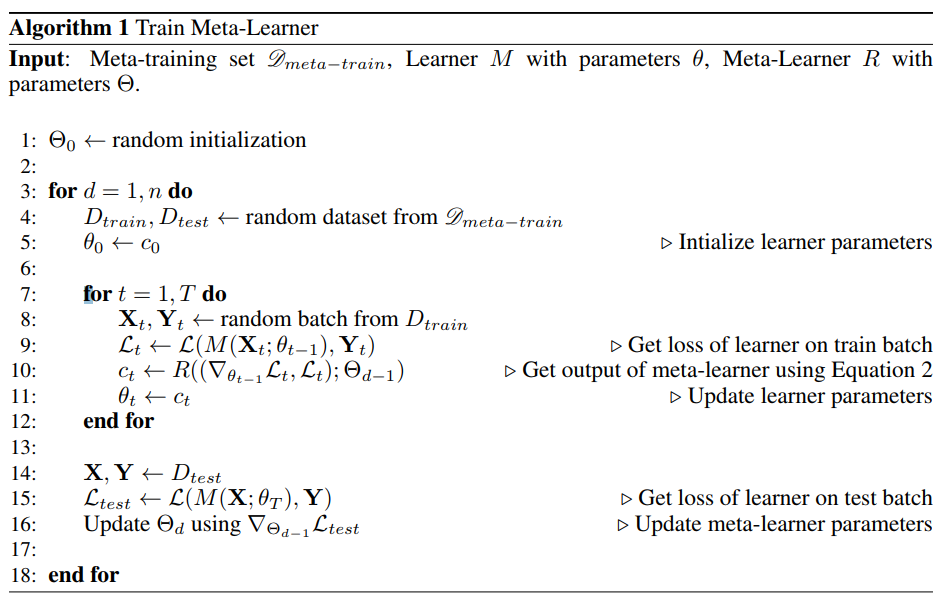
\includegraphics[scale=0.35]{/home/alex/python/D'yakonov/lstm_meta_alg.png}
\caption{{\footnotesize  Алгоритм обучения Meta-Learner}}
\end{center}
\end{figure}

\end{frame}

\begin{frame}\frametitle{Optimization as a model for few-shot learning}
\begin{figure}[h]
\begin{center}
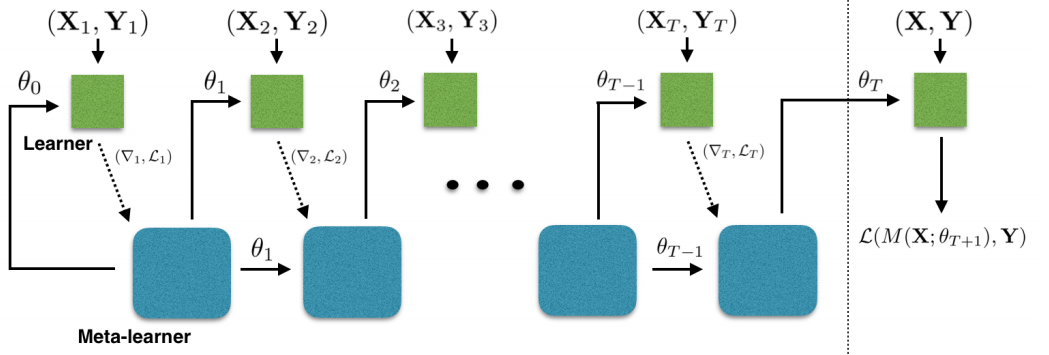
\includegraphics[scale=0.4]{/home/alex/python/D'yakonov/lstm_meta_simpl.png}
\caption{{\footnotesize  Проход вперед(forward pass) meta learner'a. Как видно часть стрелок пунктирные, это означает, что во время обновления весов эти шаги не учитываются. Это позволяет избежать появления вторых производных и сильно упрощает вычисления. Пунктирной линией отделены шаги на тестовой и тренировочной выборках.}}
\end{center}
\end{figure}
\end{frame}

\begin{frame}\frametitle{Limitations of meta learning}

\begin{block}{Ограничения}

Наибольшим ограничением является то, что распределение задач на тренировочной выборке должно быть тем же что и на тестовой.
Но на самом деле иногда новые задачи фундаментально отличаются от всех виденных ранее. Например если мы обучим модель математике, програмированию, чтению и т.д. сможет ли модель в результате выучить химию?

\end{block}

\end{frame}

\end{document}

